
\documentclass[\PRJWD/Thick_TQFTs_and_Quantum_Information.tex]{subfiles}

\begin{document}

\section{Parallel Field Theory}

In definition \ref{defn:sing_man_tqft}, we associated to each object a tensor
power of some algebra $A$; to each vertical $1$--morphism, the identity on $A$;
to each horizontal $1$--morphism, a linear map from a tensor power of $A$ to
another; to each $2$--morphism, a smooth family of linear maps. This data
suggests a codomain double category of our single manifold TQFT, which we define
next.


\subsection{Double Category of Finite Dimensional Vector Spaces}

We consider as the object or $0$--morphism category of the codomain double
category the monoidal category of finite-dimensional, real (or complex) vector
spaces $\FVect_{\K}$ for $\K = \R$ or $\C$. We then notice a categorification
of the collection of morphisms of this category as follows.

We consider the collection of all morphisms of $\FVect_{\K}$,
\[
  \s{L} := \set[f]{f \in \Hom_{\FVect_{\K}}(U, V), U, V \in \Ob \FVect_{\K}}
\]
as the object collection of the horizontal $1$--morphism category of our double
category. For each such map, we choose some $p \times q$ matrix representation
$[a_{ij}]$ which yields a mapping $\iota : \s{L} \to \M_{N}(\C)$, where
$\M_{\N}(\C)$ is the set of infinite complex matrices indexed by $\N \times \N$,
defined by:
\[
  \iota(a)_{ij} = \begin{cases}
    a_{ij} & 1 \leq i \leq p, 1 \leq j \leq q \\
    0      & \text{otherwise}
  \end{cases}
\]

This provides a notion of $2$--morphism for our double category under
construction. We notice that the Banach space $\s{B}$ of bounded operators on
the Hilbert space space $\ell^2(\N)$ can be seen as a subset of $\M_{\N}$, such
that $\s{L} \subset \s{B} \subset \M_{\N}$. It is well-known that $\s{B}$, being
a Banach space, is a simply-connected topological space. Now, for $a$ and $a'$
in $\s{L}$, we define a $2$--morphism to be a homomotpy class of paths $\alpha$
from $\iota(a)$ to $\iota(')$ in $\s{B}$, which we denote as
$\alpha : a \To a'$. By the fact the fundamental groupoid
$\Pi_1(\s{B})$ is a category, our $2$--morphisms have a strictly associative and
unital composition.  We note that the fundamental groupoid $\Pi_1(\s{B})$ is not
our morphism category -- it only supplies morphisms for $\s{L}$. An instance of
why the distinction is important is that a single morphism in $\Pi_1(\s{B})$
might represent morphisms between two different pairs of objects in $\s{L}$,
depending on the chosen matrix representations.

It is worthwhile observing the action of composition and tensor products of
linear maps on $2$--morphisms. We first notice that iota can be defined so that
it is multiplicative in two ways:
\[
  \iota(b \circ a) := \iota(b) \cdot \iota(a)
\]
where the right-hand-side product is the matrix product in $\M_{\N}(\C)$, and
\[
  \iota(a \tensor b) := \iota(a) \tensor \iota(b)
\]
where the $\tensor$ on the right is given by the Kronecker product. Now,
consider pairs of homotopic paths
$\alpha_1, \alpha_2 : a \To a'$ and
$\beta_1, \beta_2 : b \To b'$, where $b, a$ and $b', a'$ are
composeable pairs of linear maps. We consider the pointwise composites:
\begin{equation}\label{eqn:pointwise_comp}
  (\beta_i \circ \alpha_i)(t) := \beta_i(t) \circ \alpha_i(t), t \in [0, 1],
    i \in \set{1, 2}
\end{equation}
Now, the $\beta_i \circ \alpha_i$ are clearly paths
$b \circ a \To b' \circ a'$ in $\s{B}$-- we wish to show that
they are homotopic, making the operation well-defined on homomotopy classes of
paths. It suffices to observe that $\s{B}$ is simply connected, so that there is
exactly one class of homotopic paths between two points in $\Pi_1(\s{B})$.

Consider again elements
$a : U \to V, a' : U' \to V', b : X \to Y, b' : X' \to Y'$ of $\s{L}$. We define
\[
  n_x := \dim \dom x, m_x := \dim \codom x, x \in \set{a, a', b, b'}
\]
and
\[
  N_{x} = N_{x'} := \max\set{n_x, n_{x'}},
  M_{x} = M_{x'} := \max\set{m_x, m_{x'}}, x \in \set{a, b}
\]
We then have matrix representations of each $x \in \set{a, a', b, b'}$:
\[
  \iota'(x) := [\iota(x)_{ij}] \in \M_{M_x \times N_x}(\C)
\]
Now, $\M_{M_x \times N_x}(\C)$, being simply connected, has a path
$\gamma_x$ from $\iota'(x)$ to $\iota'(x')$ for each $x \in \set{a, b}$. In
fact, using the inclusion $\M_{M_x \times N_x}(\C) \hto \s{B}$ induced by
$\iota$, each $\gamma_x$ yields a path $\wh{\gamma_x}$ in $\s{B}$ from
$\iota(x)$ to $\iota(x')$, with its image contained in $\s{L}$. Since $\s{B}$ is
simply connected, every path in $\s{B}$ from $\iota(x)$ to $\iota(x')$ is
homotopic to $\wh{\gamma_x}$. Furthermore,
$\wh{\gamma_a}(t) \tensor \wh{\gamma_b}(t)$ is also a path from
$\iota(a \tensor a') = \iota(a) \tensor \iota(a')$ to
$\iota(b \tensor b') = \iota(b) \tensor \iota(b')$ in $\s{B}$, to which all
other paths with the same endpoints are homotopic. This shows that
\[
  (\wh{\gamma_a} \tensor \wh{\gamma_b})(t) :=
    \wh{\gamma_a}(t) \tensor \wh{\gamma_b}(t)
\]
is well-defined on homotopy classes of paths in $\Pi_1(\s{B})$. For
associativity of $\tensor$, we observe that
\[
  \iota(a \tensor (b \tensor c))
    = \iota(a) \tensor \iota(b) \tensor \iota(c)
    = \iota((a \tensor b) \tensor c)
\]
so that the constant path on $\iota(a) \tensor \iota(b) \tensor \iota(c)$
functions as the associator
\[
  a \tensor (b \tensor c) \to (a \tensor b) \tensor c
\]
For unitality of $\tensor$, we take the matrix $1_{\tensor} \in \s{B}$ whose
$(i, j)$ entry is $1$ if $i = j = 1$ and is $0$ otherwise, and then we observe:
\[
  \iota(a \tensor \id_{\K}) = \iota(a) \tensor 1_{\tensor} = \iota(a)
    = \iota(\id_{\K} \tensor a)
\]
so that the constant path on $\iota(a)$ functions as a left and right unitor.

We then take horizontal composition to be given by composition of linear maps
which is strictly associative and unital, with coherence following from that in
the category of vector spaces. The source and target functors are obvious -- we
send each linear map to its domain and codomain respectively. The unit functor
is also obvisous -- we send each object to its identity linear map.
%The axioms of a monoidal double category given in the unpacked version of
%definition 2.9 in \cite[5]{SymMonBicat} are also easily verified.

We compile these results into the following definition:
\begin{defn}[Double Category of Finite Dimensional Vector Spaces]
The following data form a monoidal double category:
\begin{enmrt}
\li Object category: $\FVect_{\K}$
\li Morphism category: $\s{L}$
\li Source functor: $\dom : (f : X \to Y) \mapsto X$
\li Target functor: $\codom : (f : X \to Y) \mapsto Y$
\li Unit functor: $V \mapsto \id_V$
\li Horizontal composition: $(g, f) \mapsto g \circ f$
\li Horizontal composition associator: constant path on
$\iota(a \circ b \circ c)$
\li Horizontal composition unitor: constant path on $\iota(\id_V)$, for a vector
space $V$
\li Monoidal product: $\tensor$ in appropriate contexts defined above
\li Monoidal unit: $\K$ for the object category and $\id_{\K}$ for the morphism
category
\li Monoidal associators: constant path on
$\iota(a) \tensor \iota(b) \tensor \iota(c)$ as an associator
\[
  a \tensor (b \tensor c) \to (a \tensor b) \tensor c
\]
\li Monoidal unitor: constant path on $\iota(\id_{\K}) = 1_{\tensor}$
\end{enmrt}
This is called the monoidal double category of finite dimensional $\K$--vector
spaces and is denoted $\FFVect_{\K}$.
\end{defn}

We finally note that if the choice of matrix representations poses foundational
problems, we can easily switch to the skeleton of $\FVect_{\K}$ consisting of
the spaces $\K^n$ for all $n \in \N$.

%\begin{enmrt}
%
%\li The object category is easily seen to be a monoidal category -- it is the
%monoidal category generated by a single object $A$ in a monoidal category (of
%vector spaces) and associators and unitors between its monoidal products.
%
%The morphism category consists of linear maps of the form:
%\[
%  a : A^{\tensor n} \to A^{\tensor m} \text{ and }
%  b : A^{\tensor n'} \to A^{\tensor m'}
%\]
%with some parenthesizing pattern for each domain or codomain tensor power. The
%tensor product $a \tensor b$ gives the object function of the monoidal product
%functor. The pointwise tensor product \ref{eqn:pointwise_tensor} is the morphism
%function of the monoidal product functor.
%
%\li The monoidal unit of the object category is the base field, say $\C$, and
%the unit horizontal $1$--morphism is also the monoidal unit for horizontal
%$1$--morphisms:
%\[
%  a \tensor 1_{\C} = a = 1_{\C} \tensor a
%\]
%\end{enmrt}




\subsection{Thick Tangles and Transport Graphs}

Having established a codomain double category, we look towards extending our
notion of TQFTs based on transport graphs in a single manifold to transport
graphs in cobordisms equipped with connections. For simplicity, we only consider
thick tangles equipped with connections, at the moment. Recall that a thick
tangle $X \to Y$ is a smooth surfaces $M$ with boundary $W_0 \amalg W_1$ with
equipped with smooth maps $a_M : X \to M, b_M : Y \to M$ such that $a_M$ and
$b_M$ are diffeomorphisms onto $W_0$ and $W_1$ respectively, and an embedding
$d_M : M \to \R \times [0, 1]$ (satisfying some additional properties, which we
will not need at the moment).

We consider the generating thick tangles equipped with transport graphs.
The following examples of transport graphs in the pair-of-pants, cap and their
duals gives us an idea of the structures we are dealing with:
\[
% Pants:
\begin{tikzpicture}[scale=0.55]
\pants{0, 0}
\lblvert{0, -4}{pants}{\footnotesize pair-of-pants}
\colvert{blue}{-2, 6}{a1}
\lblvert{-2.85, 6}{a1l}{\footnotesize $a_1$}
\colvert{blue}{-2, 4}{a2}
\lblvert{-2.85, 4}{a2l}{\footnotesize $a_2$}
\colvert{blue}{2, 5}{a3}
\lblvert{2.85, 5}{a3l}{\footnotesize $a_3$}
\midarrow{a1}{a3}
\midarrow{a2}{a3}
% Path 1 --> 3
\colvert{blue}{-1.55, 1.65}{a1p}
\lblvert{-1.55, 2.1}{a1pl}{\footnotesize $a_1$}
\colvert{blue}{1.5, -0.75}{a3p1}
\lblvert{1.5, -0.3}{a3p1l}{\footnotesize $a_3$}
\midarrowc{a1p}{0, 1}{0, -1}{a3p1};
% Path 2 --> 3
\colvert{blue}{-1.25, -1.95}{a2p}
\lblvert{-1.25, -1.45}{a2pl}{\footnotesize $a_2$}
\colvert{blue}{1.25, 0.35}{a3p2}
\lblvert{1.25, 0.75}{a3p2l}{\footnotesize $a_3$}
\midarrowc[0.35]{a2p}{0, -2}{1, 0.25}{a3p2}
\end{tikzpicture}
\qquad
% Cap:
\begin{tikzpicture}[scale=0.55]
\capcob{0, 0}
\lblvert{-1.5, -4}{caplbl}{\footnotesize cap}
\colvert{blue}{-2, 5}{a1}
\colvert{green!55!black}{-1, 5}{a2}
\midarrow{a1}{a2}
% Path 1 --> 2
\colvert{blue}{-1.75, 0.75}{a1p}
\colvert{green!55!black}{-1.35, -0.45}{a2p}
\midarrowc{a1p}{-1.75, -0.05}{-1, 0}{a2p}
\end{tikzpicture}
\qquad
% Cup:
\begin{tikzpicture}[scale=0.55]
\cupcob{0, 0}
\lblvert{1.5, -4}{caplbl}{\footnotesize cup}
\colvert{green!55!black}{1, 5}{a1}
\colvert{blue}{2, 5}{a2}
\midarrow{a1}{a2}
% Path 1 --> 2
\colvert{green!55!black}{1.75, 0.75}{a1p}
\colvert{blue}{1.75, -0.75}{a2p}
\midarrowc{a1p}{1.1, 0}{1.1, 0}{a2p}
\end{tikzpicture}
\qquad
% Copants
\begin{tikzpicture}[scale=0.55]
\copants{0, 0}
\lblvert{0, -4}{copants}{\footnotesize co-pair-of-pants}
\colvert{blue}{2, 6}{a1}
\lblvert{2.85, 6}{a1l}{\footnotesize $a_1$}
\colvert{blue}{2, 4}{a2}
\lblvert{2.85, 4}{a2l}{\footnotesize $a_2$}
\colvert{blue}{-2, 5}{a3}
\lblvert{-2.85, 5}{a3l}{\footnotesize $a_3$}
\midarrow{a3}{a1}
\midarrow{a3}{a2}
% Path 3 --> 1
\colvert{blue}{-1.25, 0}{a3p}
\lblvert{-1.25, 0.45}{a3pl}{\footnotesize $a_3$}
\colvert{blue}{1.5, 1.75}{a1p}
\lblvert{1.5, 2.25}{a1pl}{\footnotesize $a_1$}
\midarrowc{a3p}{0, 0}{-0.5, 1}{a1p}
% Path 3 --> 2
\colvert{blue}{1.5, -1.75}{a2p}
\lblvert{1.5, -2.25}{a2pl}{\footnotesize $a_2$}
\midarrowc{a3p}{0, 0}{-0.5, -1}{a2p}
\end{tikzpicture}
\]
We recall that edges that share an end-point need not map to paths that share an
end-point, as we see in the left diagram. At the same time, paths are allowed to
intersect. We also note that we have chosen the pretransport graphs so as to
match their sources and targets with the sources and targets of their realizing
cobordisms. We now turn our attention to the cylinder. We observe that the
cylinder is a cobordism $I \to I$. On the transport graph side, morphisms from a
single blue vertex to another can be any path with blue end-points including the
path consisting of a single blue vertex. However, the gluing unit for the single
blue vertex, on either side, is the single blue vertex itself. Hence, we will
consider the following transport graphs in the cylinder:
\[
\begin{tikzpicture}[scale=0.55]
\idcob{0, 0}
\colvert{blue}{0, 2}{a}
\lblvert{0, -2}{lbl}{\footnotesize cylinder without paths}
\end{tikzpicture}
\qquad \qquad
\begin{tikzpicture}[scale=0.55]
\idcob{0, 0}
\lblvert{0, -2}{lbl}{\footnotesize cylinder with paths}
\colvert{blue}{-2, 2}{a1}
\colvert{blue}{2, 2}{a2}
\midarrow{a1}{a2}
\colvert{blue}{-1.5, -0.15}{a1p}
\colvert{blue}{1.5, 0.15}{a2p}
\midarrowc{a1p}{0, 0.45}{0, -0.45}{a2p}
\end{tikzpicture}
\]

\begin{exm}
We take the example from our first description of the double categorical
approach and adapt it to this setting. The following is one possible diagram:
\[\begin{tikzpicture}[scale=0.33]

\idcobup{1, 0}
\colvert{blue}{-0.5, -1.85}{s}
\colvert{blue}{2, 0.25}{t}
\midarrowc{s}{0, -2}{2, -1}{t}

\coordinate (cntr) at (1, 4);
\pants{cntr}
\colvert{blue}{$(cntr) + (-1.5, 2)$}{s1}
\colvert{blue}{$(cntr) + (-1.5, -2)$}{s2}
\colvert{blue}{$(cntr) + (1.25, 0)$}{t}
\midarrowc{s1}{$(cntr) + (0, 2)$}{$(cntr) + (0, 0)$}{t}
\midarrowc{s2}{$(cntr) + (0, 1)$}{$(cntr) + (0, -1)$}{t}

\coordinate (cntr) at (5, 2);
\pants{cntr}
\colvert{blue}{$(cntr) + (-1.5, 2)$}{s1}
\colvert{blue}{$(cntr) + (-1.5, -2)$}{s2}
\colvert{blue}{$(cntr) + (1.25, 0)$}{t}
\midarrowc{s1}{$(cntr) + (0, 2)$}{$(cntr) + (0, 0)$}{t}
\midarrowc{s2}{$(cntr) + (0, 1)$}{$(cntr) + (0, -1)$}{t}

\coordinate (cntr) at (9, 2);
\begin{scope}[rotate around={180:(cntr)}]
\pants{cntr}
\colvert{blue}{$(cntr) + (-1.5, 2)$}{s1}
\colvert{blue}{$(cntr) + (-1.5, -2)$}{s2}
\colvert{blue}{$(cntr) + (1.25, 0)$}{t}
\midarrowc{s1}{$(cntr) + (0, 2)$}{$(cntr) + (0, 0)$}{t}
\midarrowc{s2}{$(cntr) + (0, 1)$}{$(cntr) + (0, -1)$}{t}
\end{scope}

\coordinate (cntr) at (13, 2);
\pants{cntr}
\colvert{blue}{$(cntr) + (-1.5, 2)$}{s1}
\colvert{blue}{$(cntr) + (-1.5, -2)$}{s2}
\colvert{blue}{$(cntr) + (1.25, 0)$}{t}
\midarrowc{s1}{$(cntr) + (0, 2)$}{$(cntr) + (0, 0)$}{t}
\midarrowc{s2}{$(cntr) + (0, 1)$}{$(cntr) + (0, -1)$}{t}

\coordinate (cntr) at (17, 2);
\begin{scope}[rotate around={180:(cntr)}]
\pants{cntr}
\colvert{blue}{$(cntr) + (-1.5, 2)$}{s1}
\colvert{blue}{$(cntr) + (-1.5, -2)$}{s2}
\colvert{blue}{$(cntr) + (1.25, 0)$}{t}
\midarrowc{s1}{$(cntr) + (0, 2)$}{$(cntr) + (0, 0)$}{t}
\midarrowc{s2}{$(cntr) + (0, 1)$}{$(cntr) + (0, -1)$}{t}
\end{scope}

\coordinate (cntr) at (21, 2);
\pants{cntr}
\colvert{blue}{$(cntr) + (-1.5, 2)$}{s1}
\colvert{blue}{$(cntr) + (-1.5, -2)$}{s2}
\colvert{blue}{$(cntr) + (1.25, 0)$}{t}
\midarrowc{s1}{$(cntr) + (0, 2)$}{$(cntr) + (0, 0)$}{t}
\midarrowc{s2}{$(cntr) + (0, 1)$}{$(cntr) + (0, -1)$}{t}

\coordinate (cntr) at (25, 2);
\begin{scope}[rotate around={180:(cntr)}]
\pants{cntr}
\colvert{blue}{$(cntr) + (-1.5, 2)$}{s1}
\colvert{blue}{$(cntr) + (-1.5, -2)$}{s2}
\colvert{blue}{$(cntr) + (1.25, 0)$}{t}
\midarrowc{s1}{$(cntr) + (0, 2)$}{$(cntr) + (0, 0)$}{t}
\midarrowc{s2}{$(cntr) + (0, 1)$}{$(cntr) + (0, -1)$}{t}
\end{scope}

\end{tikzpicture}\]
\end{exm}

\begin{exm}
We need not consider transport graphs that match the pair-of-pants or the
cylinder (or their duals) exactly. For instance, we could consider the following
graph:
\[\begin{tikzpicture}[scale=0.5]
\coordinate (cntr) at (1, 4);
\pants{cntr}
\colvert{blue}{$(cntr) + (-1.5, 2)$}{s1}
\colvert{blue}{$(cntr) + (-1.5, -2)$}{s2}
\colvert{green!55!black}{$(cntr) + (0, 1)$}{t1}
\colvert{blue}{$(cntr) + (0, -1)$}{t2}
\colvert{blue}{$(cntr) + (1.5, -0.5)$}{t3}
\midarrowc{s1}{$(cntr) + (0, 2)$}{$(cntr) + (-1, 1)$}{t1}
\midarrowc[0.33]{s2}{$(cntr) + (-0.25, -1)$}{$(cntr) + (0, 1)$}{t1}
\midarrowc{s1}{$(cntr) + (-0.5, 0)$}{$(cntr) + (-0.5, 2)$}{t2}
\midarrowc{s2}{$(cntr) + (-0.5, -2)$}{$(cntr) + (-0.5, -1)$}{t2}
\midarrowc{t1}{$(cntr) + (0.5, 0)$}{$(cntr) + (1, 0.5)$}{t3}
\midarrowc{t2}{$(cntr) + (0.5, 0.5)$}{$(cntr) + (1, -0.5)$}{t3}
\end{tikzpicture}\]
Notice that the source and target of the graph matches the source and target of
the pair-of-pants event though the graph is not a pair-of-pants graph. Also
notice that this graph has an internal green vertex.
\end{exm}

From these examples, we are motiviated to note the following definition.
\begin{defn}
Given a $2$--dimensional thick tangle, consider a transport graph in
the tangle such that the source of the graph has the same number of vertices
as the number of boundary components of the source of the tangle and the
colouring and ordering of the source of the graph is such that a blue vertex
corresponds to an interval boundary component and a green vertex corresponds to
an empty boundary component. Furthermore, that the analogous statement holds for
the targets of the graph and the tangle. We then call the given transport graph
admissible for the given tangle.
\end{defn}

An immediate corollary of this definition is:
\begin{cor}
Admissible transport graphs in gluable thick tangles are gluable.
\end{cor}

The examples we have seen so far are all admissible. We also show graphs that
are not admissible in the following example.

\begin{exm}
The following are not admissible transport graphs:
\[\begin{tikzpicture}[scale=0.33]

\coordinate (cntr) at (1, 4);
\pants{cntr}
\colvert{blue}{$(cntr) + (-1.5, 2)$}{s}
\colvert{blue}{$(cntr) + (1.5, 0)$}{t}
\midarrow{s}{t}
\lblvert{$(cntr) + (0, -5)$}{lbl}{\small not enough}
\lblvert{$(cntr) + (0, -6)$}{lbl}{\small source vertices}

\coordinate (cntr) at (11, 4);
\idcob{cntr}
\colvert{green!55!black}{$(cntr) + (-1.5, 0)$}{s}
\colvert{blue}{$(cntr) + (1.5, 0)$}{t}
\midarrow{s}{t}
\lblvert{$(cntr) + (0, -5)$}{lbl}{\small source should}
\lblvert{$(cntr) + (0, -6)$}{lbl}{\small be blue}

\coordinate (cntr) at (21, 4);
\copants{cntr}
\capcob{$(cntr) + (4, 2)$}
\colvert{blue}{$(cntr) + (-1.5, 0)$}{s}
\colvert{blue}{$(cntr) + (2.5, 2)$}{t1}
\colvert{blue}{$(cntr) + (1.5, -2)$}{t2}
\midarrow{s}{t1}
\midarrow{s}{t2}
\lblvert{$(cntr) + (0, -5)$}{lbl}{\small top traget}
\lblvert{$(cntr) + (0, -6)$}{lbl}{\small should be}
\lblvert{$(cntr) + (0, -7.25)$}{lbl}{\small green}

\end{tikzpicture}\]
\end{exm}

So far, we have only shown the diagrams of surfaces with paths in these examples
but what we need to work with are surfaces equipped with bundles, connections
and transport graphs. We will now construct a monoidal double category
consisting of these structures.

Consider the monoidal double category $\CConn^V_{\DThick}$ of gluable
connections on gluable $V$--fibred (smooth or complex) bundles on
$2$--dimensional thick tangles.
For each horizontal $1$--morphism (bundle with connection) in this category, we
take all admissible transport graphs in the base of the bundle such that all
paths consist only of points internal to the base space and away from the
boundary collar over which the bundle has been made trivial.

For each gluable bundle equipped with a gluable connection and an admissible
transport graph in this manner, we take its source to be the source of the
bundle in $\CConn^V_{\DThick}$ along with the source of the transport graph.
Targets are defined similarly. The gluing units are the disjoint unions of
cylinders of the following form shown before:
\[\begin{tikzpicture}[scale=0.55]
\idcob{0, 0}
\colvert{blue}{0, 2}{a}
\lblvert{0, -2}{lbl}{\footnotesize cylinder without paths}
\end{tikzpicture}\]

Naturally, the object category consists of the sources and targets of the
horizontal $1$--morphisms and transport isomorphisms between them that are also
connection isomorphisms -- similar to the monoidal double category $\TG(M)$ of
transport graphs in a manifold $M$ defined in subsection
\ref{subsec:sing_man_tqft}. The morphism category consists of the horizontal
$1$--morphisms along with transport isomorphisms that are also connection
isomorphisms. Finally, monoidal structure is given by disjoint union, as
expected.

Having the developed the basic idea of such a monoidal double category, we avoid
going into further detail because it does not provide any additional insight. We
simply note that the structure outlined here is a monoidal double category that
can serve as the domain for a notion of (double) functorial quantum field
theory. Hence, we end this subsection with the following definition.

\begin{defn}
The monoidal double category outlined above is called the double category of
transport graphs in $2$--dimensional thick tangles over $V$ and is
denoted $\TG\br{\CConn^V_{\DThick}}$.
\end{defn}




\subsection{Parallel Field Theory}

We are now equipped with all the machinery to define our desired notion of
topological quantum field theory.

\begin{defn}[Parallel Field Theory]
Let $A$ be a $\K$--algebra for $\K = \R$ or $\C$. Then, we define the data of a
monoidal double functor
\[
  F : \TG\br{\CConn^V_{\DThick}} \to \FFVect_{\K}
\]
Each horizontal $1$--morphism in the domain is identical to one in the
double category of transport graphs in a manifold. $F$ is thus defined on
horizontal $1$--morphisms identically to the functor in definition
\ref{defn:sing_man_tqft}.

We observe that each object can be reduced to a source or target of a
pretransport graph since, by definition the copies of $I$ and $\varnothing$ are
matched up with blue and green vertices respectively. This allows us to define
$F$ on objects identically to \ref{defn:sing_man_tqft} again. It is then easy to
see that the action of $F$ on vertical $1$--morphisms and $2$--morphisms can be
adapted similarly.

A monoidal double functor $F$ defined in this way is called a parallel field
theory (on $2$--dimensional thick tangles or $\DThick$).
\end{defn}

\begin{rmk}
The ending parenthetical remark in the previous definition suggests that we can
easily consider such field theories over other cobordism categories but we will
not pursue this idea for now.
\end{rmk}

We have not yet discussed if enough useful elements of the algebra $A$ can be
accessed with a field theory of this form. After all, this was the original
issue with $1$--categorical TQFTs. We will not treat this issue in full in this
paper but we will note that the machinery we have developed so far puts no
serious restrictions on the bundles or connections we can choose over our
manifolds. What we mean by this is that given an arbitray bundle with a
connection, we can make it gluable by only modifying it in a small collar of the
boundary. The bundle and connection behave as usual over rest of the base
manifold. We hope that this will provide enough structure to ensure that enough
useful algebra elements become accessible with a parallel field theory.
Nevertheless, we will make this problem precise for future work.
One of the main questions to be answered here the following:

\begin{qstn}\label{qstn:elem_from_pt}
Given a manifold $M$ and some fixed element $a$ of a complex algebra
$A^{\tensor n}$, are there
\begin{enmrt}
\li an $A$--fibred complex bundle $E \to M$,
\li a complex linear connection $\nabla$ on $E$,
\li a transport graph $G$ in $M$ with $S(G)$ consisting of only green vertices,
$T(G)$ having $n$ blue vertices and with the paths in the geometric realization
of $G$ away from some small neighbourhood of $\partial M$,
\end{enmrt}
such that $a$ can be obtained as a linear map $\C \to A^{\tensor n}$ in
the process described in definition \ref{defn:sing_man_tqft} for horizontal
$1$--morphisms?
\end{qstn}

\begin{qstn}\label{qstn:map_from_pt}
Given a manifold $M$ and some linear map $f : V \to V$, are there
\begin{enmrt}
\li a $V$--fibred complex bundle $E \to M$
\li a complex linear connection $\nabla$ on $E$,
\li a transport graph $G$ in $M$ with $S(G)$ and $T(G)$ both consisting of only
blue vertices, with its paths away from some neighbourhood of $\partial M$, as
before,
\end{enmrt}
such that $f$ can be obtained in the process described in definition
\ref{defn:sing_man_tqft} for horizontal $1$--morphisms?
\end{qstn}

%\TODO{Improve this statement.}

If we can answer these questions in the affirmative for a considerable
collection of elements $a \in A$, then a parallel field theory gives us a
concrete way to perform computations involving the multiplication of $A$ and
automorphisms of $A$ and tensor products of these maps, using the geometry of
manifolds. Hence, we make the following definition:

\begin{defn}
If the answers to question \ref{qstn:elem_from_pt} (or \ref{qstn:map_from_pt})
is yes for some manifold $M$, then we say that $a$ (or $f$) is accessible from
$M$.
\end{defn}

If an element $a$ is accessible from a manifold $M$, it is in the image of a
parallel field theory on $M$.
If an element $a$ is accessible from a thick tangle
$M : \varnothing \to I^{\amalg n}$ where the chosen transport graph is
admissible, then $a$ is in the image of a parallel field theory on $\DThick$.

\begin{defn}
In the latter case, we say that $a$ is accessible from $\DThick$.
\end{defn}

After this, it is easy to see
that we can compute with accessible elements using the machinery of a parallel
field theory. This picture will become clearer as we treat quantum information
and computing in the next subsection.




\subsection{Quantum Computing with Parallel Transport}

Take $A$ to be the complex matrix algebra $\M_2(\C)$ of $2 \times 2$ complex
matrices with the usual multiplication. Let
$\mathcal{U} = \set{u_1, \dots, u_n}$ be a set
of single qubit quantum gates -- unitary matrices -- in $\M_2(\C)$ such that
each $u_k$ is accessible from $\DThick$. Let the thick tangle with a bundle,
a connection and an admissible transport graph that realizes the accessibility
of the $u_k$ be $M_k$, for each $i \in \set{k, \dots, n}$.

We recall that, in the simplest terms, a quantum circuit is a sequence of
composeable complex linear unitary maps
$U_i : (\C^2)^{\tensor N} \to (\C^2)^{\tensor N}$, $i = 1, \dots, p$.
For simplicity, we assume that
each $U_i$ arises as a tensor product $\bigotimes_{j = 1}^{N} g_{i, j}$ for
gates $g_{i, j} \in \mathcal{U}$. Since each $g_{i, j}$ is accessible, we have
a $G_{i, j} \in \set[M_k]{k = 1, \dots, n}$ such that $F(G_{i, j}) = g_{i, j}$
for a parallel field theory $F$. Then, we have:
\[
 U := U_p \circ \cdots \circ U_1
  = \bigotimes_{j = 1}^{N} g_{p, j} \circ \cdots
    \circ \bigotimes_{j = 1}^{N} g_{1, j}
  = \bigotimes_{j = 1}^{N} (g_{p, j} \circ \cdots \circ g_{1, j})
\]
where $\circ$ is matrix multiplication (composition of linear maps). Consider
the following transport graph in the pair-of-pants:

\[\begin{tikzpicture}[scale=0.25]
\pants{1, 0}
\colvert{blue}{-1, 6}{s1}
\colvert{blue}{-1, 4}{s2}
\colvert{blue}{3, 5}{t}
\colvert{blue}{1, 0}{a}
\midarrow{s1}{t}
\midarrow{s2}{t}
\end{tikzpicture}\]
where each edge is geometrically realized as a constant path on a single point
-- shown as a blue dot -- in the pair-of-pants. This graph is admissible and
provides a binary operation on thick tangles with target $I$ in the obvious way.
We denote this operation as $\wedge$. It is then easy to see that
\[
  U = F\br{\coprod_{j = 1}^{N} G_{p, j} \wedge \cdots \wedge G_{1, j}}
\]
We should stress that $\wedge$ is not associative, even up to isomorphism, in
$\DThick$ but its image under $F$ is. The reason for failure of associativity is
that graphs do not have the smooth structure needed for associator isomorphisms
for $\wedge$.

This setup provides a very basic formalism for expressing quantum
circuits in the language of thick tangles equipped with bundles, connections and
transport graphs.
We note, however, that it is not clear what structure plays the role of
qubits or registers in this picture. One easy way to get around this is to
consider the following embedding of $\C^2$ into $\M_2(\C)$:
\[
  \bmat{a \\ b} \mapsto \bmat{a & 0 \\ b & 0}
\]
If we then require that the following matrices are accessible:
\[
  \bmat{1 & 0 \\ 0 & 0} \text{ and } \bmat{0 & 0 \\ 1 & 0}
\]
we can model classical inputs with thick tangles just like gates. Multiplying
inputs with circuits using the pair-of-pants then models the application of
the circuit to the input.

One issue with this approach is that there might be gates acting on more
than one qubit that are not elementary tensor products of single qubit gates.
For instance, the controlled not gate is one such example. In order to obtain
non-elementary tensors, we will addition of vectors. To capture this in the
language of parallel field theories, we need a notion of addition for
cobordisms. We will return to this idea in the next subsection. For now, we
observe another approach to quantum computing using parallel field theories.

We now take the fibres of our bundles to be $\C^2$ -- the space where a single
qubit lives (recall \ref{rmk:any_vect_space}).
We then assume that our previous collection of quantum gates in
$\C^2 \to \C^2$ are accessible from a collection of $2$--dimensional thick
tangles $G'_{i, j} : I \to I$ (not $\varnothing \to I$, this time) such that
$F(G'_{i, j}) = g_{i, j}$. Then, the quantum circuit can be expressed as:
\[
  U = F\br{\coprod_{j = 1}^{N} G'_{p, j} * \cdots
           * \coprod_{j = 1}^{N} G'_{1, j}}
\]
recalling that $*$ is gluing of thick tangles.
Notice that single qubit inputs are linear maps $\C \to C^2$. Hence, we now
assume that linear maps
\[
  \ket{0} = z \mapsto z\bmat{1 \\ 0} \text{ and }
  \ket{1} = z \mapsto z \bmat{0 \\ 1}
\]
are accessible. That is, a quantum register is a disjoint union of thick tangles
$\mathbf{0}, \mathbf{1} : \varnothing \to I$ realizing $\ket{0}$ and $\ket{1}$
respectively.

It is then easy to see that an application of a quantum circuit to quantum
register is given by composition of thick tangles.





\subsection{Addition of Cobordisms}

We now make precise the notion of addition for $2$--dimensional thick tangles
mentioned in the previous subsection, so that non-elementary tensors become
accessible with parallel field theories.

Consider $2$--dimensional thick tangles $M : I^{\amalg n} \to I^{\amalg m}$ and
$N : I^{\amalg n'} \to I^{\amalg m'}$. Suppose $S_1 \in \set{S(M), S(N)}$ is the
source of either $M$ or $N$ with the most copies of $I$ and $S_0$ is that with
the least copies of $I$. $T_0, T_1 \in \set{T(M), T(N)}$ are defined
analogously. That is, $S_0 = I^{\amalg \min\set{m, m'}}$,
$T_0 = I^{\amalg \min\set{n, n'}}$, $S_1 = I^{\amalg \max\set{m, m'}}$ and
$T_1 = I^{\amalg \max\set{n, n'}}$. Then, $M + N$ is defined to be the shape
obtained by gluing $S_0$ to the first $\min\set{m, m'}$ copies of $I$ in
$S_1$ and $T_0$ to the first $\min\set{n, n'}$ copies of $I$ in $T_1$.

For instance, let $M$ be the pair-of-pants and $N$ the cylinder $I \times I$.
Then, pictorially, $M + N$ would look like\footnote{generated using
\cite{Mathcha}}:

\[
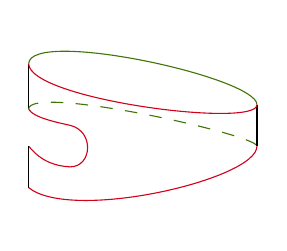
\begin{tikzpicture}[x=0.75pt,y=0.75pt,yscale=-1,xscale=1]
%Curve Lines [id:da6783491277813168]
\draw [color={rgb, 255:red, 208; green, 2; blue, 27 }  ,draw opacity=1 ]
(10,62.25) .. controls (12.6,66.54) and (25,68.8) .. (30,70) ;
%Curve Lines [id:da8932052500161816]
\draw [color={rgb, 255:red, 208; green, 2; blue, 27 }  ,draw opacity=1 ]
(10,80) .. controls (16.2,87.6) and (23,89.6) .. (30,90) ;
%Curve Lines [id:da5336367474763575]
\draw [color={rgb, 255:red, 208; green, 2; blue, 27 }  ,draw opacity=1 ]
(30,70) .. controls (41.8,72.8) and (40.6,90) .. (30,90) ;
%Straight Lines [id:da20283370527792666]
\draw (10,40.25) -- (10,62.25) ;
%Straight Lines [id:da4944370504980129]
\draw (10,80) -- (10,100) ;
%Curve Lines [id:da1547743895825433]
\draw [color={rgb, 255:red, 208; green, 2; blue, 27 }  ,draw opacity=1 ]
(10,100) .. controls (30.6,116.7) and (120.2,96) .. (120,80) ;
%Curve Lines [id:da9098653012878017]
\draw [color={rgb, 255:red, 65; green, 117; blue, 5 }  ,draw opacity=1 ]
(10,40.25) .. controls (11,23.2) and (119.8,46.8) .. (120,60) ;
%Curve Lines [id:da10875506317214012]
\draw [color={rgb, 255:red, 65; green, 117; blue, 5 }  ,draw opacity=1 ]
[dash pattern={on 4.5pt off 4.5pt}]  (10,62.25) .. controls (9.8,50) and
(119.8,74.4) .. (120,80) ;
%Straight Lines [id:da5956309013033436]
\draw    (120,60) -- (120,80) ;
%Curve Lines [id:da23301521900677968]
\draw [color={rgb, 255:red, 208; green, 2; blue, 27 }  ,draw opacity=1 ]
(10,40.25) .. controls (10.2,57.6) and (120.6,71.6) .. (120,60) ;
\end{tikzpicture}
\]
We note that this operation is distinct from both the disjoint union and the
gluing of thick tangles end-to-end. In particular, the results of this operation
can not, in general, be embeded into the infinite strip $\R \times I$. However,
we observe that we can unambiguously define the sources and targets of these
shapes as sources $S_1$ and $T_2$ respectively. We also observe that when
the domains and codomains of the summands are the same, the picture of a sum is
simply a diagram in $\DThick$ involving parallel cobordisms. This motivates us
to name these shapes as follows.

\begin{defn}
For thick tangles $M, N, S_0, T_0, S_1, T_1$ as above, $M + N$ is called a
multitangle $S_1 \to T_1$. In particular, we take the empty manifold to be
the empty sum -- a multitangle between any pair of objects in $\DThick$.
\end{defn}

\begin{rmk}
We observe that this definition carries over as is to transport graphs, bundles
and connections, even though the results of this kind of addition need not be
transport graphs, bundles or connections. In fact, if we take sums of three
cobordisms, then the result might even fail to be a manifold.
\TODO{Is it still a manifold?} Nevertheless, we will carry on with this
construction, being aware that we might start to lose some of the double
categorical structures.
\end{rmk}

However, we will observe that many of the useful structures in $\DThick$ are not
disturbed by this operation. We first define the starting data of yet another
double category:

\begin{enmrt}
\li Object category: same as $\TG\br{\CConn^V_{\DThick}}$
\li Morphism category: objects are sums of objects in
$\TG\br{\CConn^V_{\DThick}}$, including the empty sum, and morphisms are
piecewise isomorphisms -- that is, they are tuples of $2$--morphisms in
$\TG\br{\CConn^V_{\DThick}}$, one for each summand
\end{enmrt}

We would like to make our structure resemble an additive category. For this, we
will modify the definition of end-to-end gluing or horizontal composition so as
to make it bi-$\Z$--linear as follows. First, we will reduce diagrams involving
multibordisms into line diagrams of the following form, for simplicity:
\[\begin{tikzpicture}
\colvert{black}{1, 0}{s}
\colvert{black}{3, 0}{t}
\path
  (s) edge[bend left] (t)
  (s) edge (t)
  (s) edge[bend right] (t)
  ;
\end{tikzpicture}\]
where we shrink sources and targets to single vertices. Now, suppose that we
have thick tangles $M_i : X \to Y, i \in \set{1, \dots, m}$ and
$N_j : Y \to Z, j \in \set{1, \dots, n}$. Then, we can define
\[
  \sum_{j = 1}^n N_j * \sum_{i = 1}^m M_i
  := \sum_{i = 1}^n \sum_{j = 1}^m N_j * M_i
\]
since the relevant composites all exist. For $m = 3, n =2$, in line diagrams,
this equation is:
\[\begin{tikzpicture}
\colvert{black}{1, 0}{X}
\colvert{black}{3, 0}{Y}
\lblvert{3.5, 0}{glue}{$\cdots$}
\colvert{black}{4, 0}{YY}
\colvert{black}{6, 0}{Z}
\path
  (X)  edge[bend left=70]   node[above]{$M_1$}   (Y)
  (X)  edge                 node[above]{$M_2$}   (Y)
  (X)  edge[bend right=70]  node[below]{$M_3$}   (Y)
  (YY) edge[bend left]      node[above]{$N_1$}   (Z)
  (YY) edge[bend right]     node[below]{$N_2$}   (Z)
  ;
\lblvert{6.5, 0}{equals}{$:=$}
\colvert{black}{7, 0}{XX}
\colvert{black}{11, 0}{ZZ}
\draw
  (XX) to[bend left=90]
  node[midway, draw=black, fill=black, shape=circle, inner sep=\vertinnersep]{}
  node[midway, above]{{\footnotesize $N_1 * M_1$}}
  (ZZ);
\draw
  (XX) to[bend left=35]
  node[midway, draw=black, fill=black, shape=circle, inner sep=\vertinnersep]{}
  node[midway, above]{{\footnotesize $N_1 * M_2$}}
  (ZZ);
\draw
  (XX) to[bend left=10]
  node[midway, draw=black, fill=black, shape=circle, inner sep=\vertinnersep]{}
  node[midway, above]{{\footnotesize $N_1 * M_3$}}
  (ZZ);
\draw
  (XX) to[bend right=10]
  node[midway, draw=black, fill=black, shape=circle, inner sep=\vertinnersep]{}
  node[midway, below]{{\footnotesize $N_2 * M_1$}}
  (ZZ);
\draw
  (XX) to[bend right=35]
  node[midway, draw=black, fill=black, shape=circle, inner sep=\vertinnersep]{}
  node[midway, below]{{\footnotesize $N_2 * M_2$}}
  (ZZ);
\draw
  (XX) to[bend right=90]
  node[midway, draw=black, fill=black, shape=circle, inner sep=\vertinnersep]{}
  node[midway, below]{{\footnotesize $N_2 * M_3$}}
  (ZZ);
\end{tikzpicture}\]
In other words, during horizontal composition of multitangles, we first undo
the gluing resulting from addition at the composition site, duplicate the
branches as needed and then perform the gluing for horizontal composition. This
new gluing operation is easily seen to be associative up to piecewise
isomorphisms. Furthermore, we have
\[
  (N_1 + N_2) * M_1 = (N_1 * M_1) + (N_2 * M_1)
\]
In pictures:
\[\begin{tikzpicture}
\colvert{black}{1, 0}{X}
\colvert{black}{3, 0}{Y}
\lblvert{3.5, 0}{glue}{$\cdots$}
\colvert{black}{4, 0}{YY}
\colvert{black}{6, 0}{Z}
\path
  (X)  edge   node[above]{$M_1$}   (Y)
  (YY) edge[bend left]   node[above]{$N_1$}  (Z)
  (YY) edge[bend right]  node[below]{$N_2$} (Z)
  ;
\lblvert{6.5, 0}{equals}{$:=$}
\colvert{black}{7, 0}{XX}
\colvert{black}{9, 0.30}{YYY}
\colvert{black}{9, -0.30}{YYYY}
\colvert{black}{11, 0}{ZZ}
\draw (XX) .. controls (7.5, 0.25) and (8.5, 0.30) .. (YYY);
\draw (YYY) .. controls (9.5, 0.30) and (10.5, 0.25) .. (ZZ);
\draw (XX) .. controls (7.5, -0.25) and (8.5, -0.30) .. (YYYY);
\draw (YYYY) .. controls (9.5, -0.30) and (10.5, -0.25) .. (ZZ);

\lblvert{9, 0.55}{NM}{$N_1 * M_1$}
\lblvert{9, -0.55}{NNMM}{$N_2 * M_1$}
\end{tikzpicture}\]
If, in addition, $M_1 = Y \times I$, then we easily see that there is a
piecewise isomorphism $(N_1 + N_2) * M_1 \to N_1 + N_2$. It also easy to see for
arbitrarily many $N_1, \dots, N_n$ -- that is, horizontal
composition is right unital up to isomorphism. Left unitality is similar --
consider $N_1 * (M_1 + M_2)$ and take $N_1 = Y \times I$. We should note that
the addition of (multi-)cobordisms does not have immediate inverses but it is
commutative up to piecewise isomorphism. Hence, the morphism category of
multitangles is an up-to-isomorphism commutative monoid.

So far, we have defined addition on horizontal $1$--morphisms. We will define
addition on objects to fit this picture. Given $I^{\amalg m}$ and
$I^{\amalg m'}$, we define
\[
  I^{\amalg m} + I^{\amalg m'} := I^{\amalg \max\set{m, m'}}
\]
Without strictly verifying (or even defining) axioms further, we propose that
multitangles form a structure akin to an additive double category with
monoidal structure (given by disjoint union) -- in some loose sense, at the very
least. We invite the reader to formulate this notion of double category with
fully defined axioms to make our structure fit the definition.

We then move on to show that with this structure we have a more robust notion of
field theory capable of handling non-elementary tensors in the context of
quantum computing. To this end, we define:

\begin{defn}
We denote the ``additive monoidal double category'' of multitangles constructed
so far as $\TG^+(\CConn^V_{\DThick})$.
\end{defn}




\subsection{Quantum Computing Revisited}

Given a parallel field theory as defined so far, we can extend the domain of
$F$ to the structure $\TG^+\br{\CConn^V_{\DThick}}$ in an obvious way to obtain
a ``functor'' $F^+$ as follows. $F^+$ is identical to $F$ on the object category
-- there are no issues here since the object category was not modified in
constructing $\TG^+\br{\CConn^V_{\DThick}}$. A horizontal $1$--morphism in this
``double category'', however, is of the form
\[
  M = M_1 + \cdots + M_k
\]
for horizontal $1$--morphisms $M_i, i \in \set{1, \dots, k}$ in
$\TG\br{\CConn^V_{\DThick}}$. $F^+(M)$ is defined to be
\[
  F^+(M) := F(M_1) + \cdots + F(M_k)
\]
where the addition on the right is not well-defined as is. To define this we
observe that that each $F^+(M_i)$ is a linear map
$F(I)^{\tensor n_i} \to F(I)^{\tensor m_i}$. Then, we choose a sensible
embedding of each $F(I)^{\tensor n_i}$ in $F(I)^{\tensor \max_i n_i}$ and of
each $F(I)^{\tensor m_i}$ in $F(I)^{\tensor \max_i m_i}$. After this, the
addition is taken within within the space of linear maps
$F(I)^{\tensor \max_i n_i} \to F(I)^{\tensor \max_i m_i}$. We also note that if
$M = \varnothing$, then we define:
\[
  F(M)(x) := 0, \forall x
\]

\begin{defn}
An additive parallel field theory is an ``additive monoidal double functor''
\[
  F : \TG^+(\CConn^V_{\DThick}) \to \FFVect_{\C}
\]
defined using the above construction.
Accessibility is defined similarly for additive parallel field theories.
\end{defn}

Given a collection of $1$--qubit gates, we can take sums of tensor products of
these gates to obtain multi-qubit gates that are not elementary tensors.  Thus,
if we can solve the accessibility problem for $1$--qubit gates in the first
sense of parallel field theories, we can express sums of tensor products of
these gates using multitangles. Thus, we have a concrete way to express both
quantum registers and circuits using structures in $\TG^+(\CConn^V_{\DThick})$
which finally yield usual linear algebraic quantum registers and circuits under
additive parallel field theories. In fact, both approaches to quantum computing
discussed before can be adapted to this framework. It is then also easy to adapt
this notion back to the single manifold case of \ref{subsec:sing_man_tqft}.




\subsection{Operads}

Our goal in this paper was to present an elementary method to formalize quantum
computing in the language of TQFTs and geometric structures supported on them.
Hence our constructions are mostly based on combinatorial and geometric data
that can be associated with cobordisms. Nevertheless, one cannot but notice the
similarity of transport graphs and, more visibly, cobordisms themselves with
operads. As a start, consider the operad of rooted trees whose non-root vertices
are all leaves and where composition is given by gluing the root of a tree with
one of the leaves of another \cite{WhatOp}. Of course, for each leaf, we get a
different composite which is different from gluing of cobordisms, at first
sight. An example is shown below, where the subscript of the composition sign
indicates the leaf chosen for the gluing.
\[\begin{tikzpicture}

\colvert{black}{-2, 0}{a}
\colvert{black}{-3, 0.5}{a1};
\colvert{black}{-3, 0}{a2};
\colvert{black}{-3, -0.5}{a3};
\draw (a1) -- (a);
\draw (a2) -- (a);
\draw (a3) -- (a);

\lblvert{-1.5, 0}{comp}{$\circ_2$}

\colvert{black}{0, 0}{a}
\colvert{black}{-1, 0.25}{a1};
\colvert{black}{-1, -0.25}{a2};
\draw (a1) -- (a);
\draw (a2) -- (a);

\lblvert{0.5, 0}{eq}{$=$}

\colvert{black}{3, 0}{a}
\colvert{black}{2, 0.5}{a1};
\colvert{black}{2, 0}{a2};
\colvert{black}{2, -0.5}{a3};
\draw (a1) -- (a);
\draw (a2) -- (a);
\draw (a3) -- (a);

\colvert{black}{1, 0.25}{a4};
\colvert{black}{1, -0.25}{a5};
\draw (a4) -- (a2);
\draw (a5) -- (a2);

\end{tikzpicture}
\]

However, we notice that the difference of this situation with transport graphs
or cobordisms is artificial for we could define composition operations for
transport graphs and cobordisms parametrized by their inputs and outputs just as
in the case of operads. Note, however, that we need to handle the gluing of
multiple outputs to inputs in various combinations. For this, we informally
introduce a modification of operads.

\begin{defn}
Let $\s{C}$ be any (not necessarily symmetric) monoidal category and
$P = \set{P(n, m)}_{n, m \in \N}$ be a
collection of objects of $\s{C}$. For any $n \in \N$ and $1 \leq i \leq n$,
let $I = \set{i, i + 1, \dots, i + m} \subset \set{1, \dots, n}$. For each
such $n$ and $I$ as well as some $n' \in \N$, suppose there is a morphism in
$\s{C}$ as follows:
\[
  \circ_I : P(n, m) \tensor P(n', n) \to P(n', m)
\]
Then, with some coherence conditions we have not explored, we will call
$P$ a multioperad in $\s{C}$.
\end{defn}

\begin{exm}
Consider the same diagram above giving an example of operads of trees. This
diagram is an example of a (pre)transport graph if we direct the edges and
colour the vertices! The only difference is that the composition operation given
here is parametrized by a ``segment'' of the gluing site. We give another
example below:
\[\begin{tikzpicture}

\colvert{green!55!black}{1, 2.5}{c}
\colvert{blue!55!black}{1, 1.75}{cc}
\colvert{blue!55!black}{0, 3.25}{c1}
\colvert{green!55!black}{0, 2.75}{c2}
\colvert{blue!55!black}{0, 2.25}{c3}
\colvert{blue!55!black}{0, 1.75}{c4}
\midarrow{c1}{c}
\midarrow{c2}{c}
\midarrow{c3}{c}
\midarrow{c4}{c}
\midarrow{c4}{cc}

\lblvert{2, 2.5}{comp}{$\circ_{\set{2, 3}}$}

\colvert{green!55!black}{4, 3}{a}
\colvert{blue!55!black}{3, 3.5}{a1}
\colvert{blue!55!black}{3, 3}{a2}
\colvert{blue!55!black}{3, 2.5}{a3}
\midarrow{a1}{a}
\midarrow{a2}{a}
\midarrow{a3}{a}

\colvert{blue!55!black}{4, 2}{b}
\colvert{green!55!black}{3, 2}{b1}
\colvert{blue!55!black}{3, 1.5}{b2}
\midarrow{b1}{b}
\midarrow{b2}{b}
\midarrow{a3}{b}

\lblvert{5, 2.5}{comp}{$=$}

\colvert{green!55!black}{8, 2.5}{c}
\colvert{blue!55!black}{8, 1.75}{cc}
\colvert{blue!55!black}{7, 3.25}{c1}
\colvert{green!55!black}{7, 2.75}{c2}
\colvert{blue!55!black}{7, 2.25}{c3}
\colvert{blue!55!black}{7, 1.75}{c4}
\midarrow{c1}{c}
\midarrow{c2}{c}
\midarrow{c3}{c}
\midarrow{c4}{c}
\midarrow{c4}{cc}

\colvert{blue!55!black}{6, 3.5}{a1}
\colvert{blue!55!black}{6, 3}{a2}
\colvert{blue!55!black}{6, 2.5}{a3}
\colvert{green!55!black}{6, 2}{b1}
\colvert{blue!55!black}{6, 1.5}{b2}
\midarrow{a1}{c2}
\midarrow{a2}{c2}
\midarrow{a3}{c2}
\midarrow{b1}{c3}
\midarrow{b2}{c3}
\midarrow{a3}{c3}

\end{tikzpicture}\]
In this example, we considered coloured vertices and hence what we really
require is a coloured variant of multioperads, in the same spirit of introducing
colours to ordinary operads.
\end{exm}

\begin{exm}
Of course, thick tangles admit the same structure -- simply interpret the above
example in the context of thick tangles.
\end{exm}

Note, in particular, the similarity with cyclic operads as defined in
\cite{ModOp}. Recall that a cyclic operad $P$ is roughly an operad with the
action of the symmetric group $S_n$ group on $P(n)$ replaced by an action of
$S_{n + 1}$. This effectively conflates the ``inputs'' and ``outputs'' of an
operad ``element''. Here, however, we take a much more elementary approach --
simply allow multiple inputs and multiple outputs. The other difference is that
a multioperad should not require symmetry in a monoidal category for our
categories of thick tangles and transport graphs are not equipped with symmetry.
We also note a connection to modular operads \cite{ModOp}.

A modular operad is roughly a cyclic operad which allows for the gluing of
``inputs'' and ``outputs'' of the same operation \cite{Giansiracusa}.
This exact formalism is not present in the our setting, but we can introduce
something similar, although in a non-unique way. Consider the simple example
below. Here, we wish to glue the first and only output to the first input, say.
One way to accomplish this is shown on the right.
\[\begin{tikzpicture}
\colvert{green!55!black}{0, 3}{a}
\colvert{blue!55!black}{-1, 3.5}{a1}
\colvert{blue!55!black}{-1, 3}{a2}
\colvert{blue!55!black}{-1, 2.5}{a3}
\midarrow{a1}{a}
\midarrow{a2}{a}
\midarrow{a3}{a}

\draw[->] (1, 3) to (2, 3);

\colvert{blue!55!black}{5, 3}{a}
\colvert{green!55!black}{4, 3.5}{a1}
\colvert{blue!55!black}{4, 3}{a2}
\colvert{blue!55!black}{4, 2.5}{a3}
\midarrow{a1}{a}
\midarrow{a2}{a}
\midarrow{a3}{a}

\colvert{green!55!black}{3, 4}{b}
\colvert{green!55!black}{6, 4}{c}
\midarrow{b}{a1}
\midarrow{b}{c}
\midarrow{a}{c}
\end{tikzpicture}\]

We observe that these gluing constructions work as-is for the gluing
construction for bundles with connection as well so that our framework for
quantum computing could be treated in this operadic formalism but we will not
explore this idea in greater detail in this paper. Nevertheless,
these preliminary observations hint at various possibilities.
Modular operads as developed by Getzler and Kapranov generalize
Kontsevich's graph complexes \cite{ModOp}. It if of interest to fully flesh out
the connection of transport graphs to modular operads for this could lead to the
application of Chern-Simons theory to the quantum computing framework
developed in this paper. On the other hand, an approach to cobordism
theory using coloured operads \cite{CobOp} has been used to categorify $sl_n$
quantum invariants. The operadic approach to transport graphs on manifolds
with connections might be one way to relate categorification in
representation theory with quantum computing.



\subsection{Riemann Surfaces (Kontsevich)}

\TODO{Connect with Kontsevich's category.}

\subsection{Hyperbolic Band Theory}

\TODO{Connect with hyperbolic band theory paper, perhaps}

\subsection{Categorification in Representation Theory}

\TODO{Connect with Joel Kamnitzer et al.'s work on categorification.}

\end{document}

